\chapter{Implementation}

  In order to analyze how effective our attacks can steal links from the training graph of an inductive trained graph neural network, we performed several experiments by attacking GNNs that have been trained to perform node classification.
  In this chapter we want to go through the implementation of our attacks.
  We covered multiple datasets and types of graph neural network models, leading to an amount of \textasciitilde200 experiments.
  Due computational and time constraints, most of the parameters to optimize the attacks remain unexplored.

  \section{Datasets}
  \label{section:datasets}

    For all our experiments, we used 3 datasets in total.
    In the table below, they are listed with their most interesting attributes.
    All of the datasets we used are from the same domain - Citation Networks.
    This is because these networks are open source and similar to social networks in their structure.
    Due to computational constraints we didn't use social network datasets like reddit.

    \vspace{0.48cm}
    \begin{table}[!h]
      \centering
      \footnotesize
      \begin{tabular}{l|l|l|l|l}
        \toprule
        Name & Number of Nodes & Number of Edges & Number of Classes & Feature Amount \\
        \midrule
        Cora & 2708            & 5429            & 7                 & 1433 \\
        CiteSeer & 3327        & 4732            & 6                 & 3703 \\
        Pubmed & 19717         & 44338           & 3                 & 500 \\
        \bottomrule
      \end{tabular}
      \caption{Dataset Information}
      \label{table:datasets}
    \end{table}

    \subsection*{Sample Datasets for Experiments}
    \label{subsection:dataset-samples}

      In total we train target models on all three datasets - \emph{Cora}, \emph{CiteSeer} and \emph{Pubmed} .
      To train the attacker models, we sample an adversary dataset based on the incomplete subgraph.

      \subsubsection*{Same Dataset Distributions - Attack 1-2}
        Let $D_{f_t} = (V_{f_t}, E_{f_t})$ be one of our three original datasets with $|V_{f_t}|$ nodes and $|E_{f_t}|$ edges.
        We denote $D' = (V',E')$ as subgraph of $D_{f_t}$.
        $D_{f_t}$ is used to train our target model $f_t$, while $D'$ is used to sample $G_{A}$, which is a graph, that was modified by deleting some known edges to simulate an incomplete graph.
        $D_A$ is obtained by querying $f_t$ on a subgraph of $G_A$. 

        \vspace{0.48cm}
        \begin{figure}[h!]
          \begin{center}
            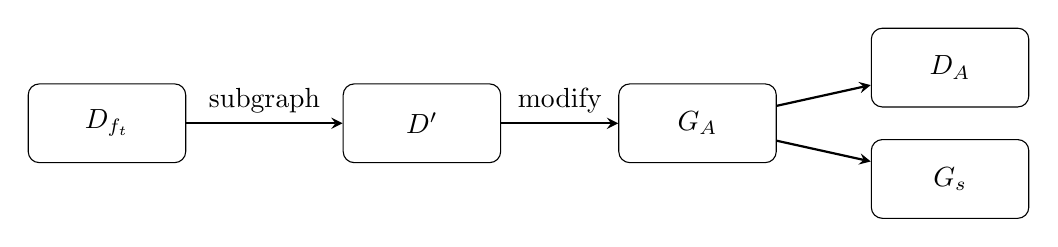
\begin{tikzpicture}
              
              % Definitions
              \tikzstyle{Dataset} = [rectangle, rounded corners,minimum width=2cm, minimum height=1cm, text centered, draw=black]
              \tikzstyle{arrow} = [thick,->,>=stealth]

              \node (Dft) [Dataset] {$D_{f_t}$};
              \node (D') [Dataset, right of=Dft, xshift=3cm] {$D'$};
              \node (GA) [Dataset, right of=D', xshift=2.5cm] {$G_A$};
              \node (DA) [Dataset, above right of=GA, xshift=2.5cm] {$D_A$};
              \node (Gs) [Dataset, below right of=GA, xshift=2.5cm] {$G_s$};

              \draw [arrow] (Dft) -- node[anchor=south] {subgraph} (D');
              \draw [arrow] (D') -- node[anchor=south] {modify} (GA);
              \draw [arrow] (GA) -- node[anchor=south] {} (Gs);
              \draw [arrow] (GA) -- node[anchor=south] {} (DA);

              

            \end{tikzpicture}
          \end{center}
          \caption{Sampling Datasets - Same Dataset Distribution - Attack 1-2}
          \label{figure:sample-datasets-attack1-2}
        \end{figure}

        We define $G_A = (V_A, E_A)$ with $V_A = V'$ and $E_A = E'$, which is now an exact copy of $D'$.
        To sample $D_A$, we first collect a set of positive samples $pos = \{(i,j, 1)$ | $\forall i,j \in V': (i,j) \in E' \wedge |pos| < ((1 - \alpha) * |E'|))\}$, containing pairs of nodes, that are connected in $D'$, where $\alpha$ denotes the percentage of known edges.
        Now, we collect a set of negative samples $neg = \{(i,j, 0)$ | $\forall i,j \in V': (i,j) \not\in E' \wedge |neg| < ((1 - \alpha) * |E'|))\}$, containing pairs of nodes, that are not connected in $D'$.
        We then delete all edges we sampled for $pos$, in our graph clone $G_A$, to simulate the missing edges, we want to steal.
        This leads to $E_A = \{(i,j)$ | $\forall (i,j) \in E': (i,j) \not\in pos\}$.
        $G_A$ is now a modified graph that contains less edges then the original graph $D'$ and we define a raw-dataset $raw = pos \cup neg$, containing the positive and negative samples obtained from $D'$.
        As the next step, we create the adversary's dataset $D_A = \{(post_{ij}, l)$ | $\forall (i,j,l)\in raw: post_{ij} = concat(f_t(G_A, i), f_t(G_A, j))\}$ for \emph{Attack 1} and $D_A = \{(dist_{ij}, l)$ | $\forall (i,j,l)\in raw: dist_{ij} = dist(post_i, post_j)\}$ for \emph{Attack 2}.
        $f_t(G_A, i)$ returns the node classification output posterior of the target model, when it is queried on $i$ given the adversary's graph $G_A$.
        $concat(a, b)$ concatenates the output posteriors $a$ and $b$ with each other returning the feature we will train the attacker model on.
        $l$ denotes the label either being 1 (positive sample) or 0 (negative sample).
        $dist(a,b) = [Cosine(a,b), ..., Sqeuclidean(a,b)]$, return the vector containing 8 different distance values like described in Section \refeq{section:threat-model}.
        With our adversary's dataset $D_A$ we can now continue training our attacker model using either $post_{ij}$ or $dist_{ij}$ as input features and $l$ as class.
        $G_s$ represents the incomplete subgraph of $D_{f_t}$, which will be used to test the adversary performance on $f_f$.
        More precisely, how well does the adversary can predict correctly whether a link between two nodes in $G_s$ is missing or not.

      \subsubsection*{Different Dataset Distributions - Attack 3}

        Let $D_{f_A}$ and $D_{f_t}$ be two of our three original datasets.
        We use $D_{f_A}$ to train the shadow model $f_A$ and $D_{f_t}$ to train our target model $f_t$.
        We denote $D_1'$ as subgraph of $D_{f_A}$ and $D_2'$ as subgraph of $D_{f_t}$.
        To sample $D_A$ we follow the same steps as described in \emph{Attack 1}.
        Firstly we create an incomplete graph $G_A$ by randomly deleting some edges.
        We then sample $D_A$ by querying $f_A$ on $G_A$.
        To obtain $G_s$ we modify $D_2'$ by randomly deleting some edges and use it to test the adversary performance on $f_t$.

        \vspace{0.48cm}
        \begin{figure}[h!]
          \begin{center}
            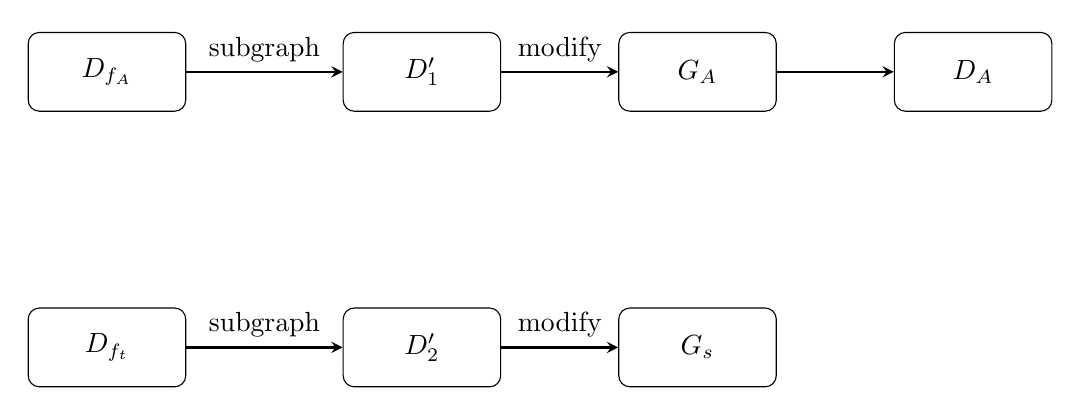
\begin{tikzpicture}
              
              % Definitions
              \tikzstyle{Dataset} = [rectangle, rounded corners,minimum width=2cm, minimum height=1cm, text centered, draw=black]
              \tikzstyle{arrow} = [thick,->,>=stealth]

              \node (Dfa) [Dataset] {$D_{f_A}$};
              \node (D1') [Dataset, right of= Dfa, xshift=3cm] {$D_1'$};
              \node (GA) [Dataset, right of= D1', xshift=2.5cm] {$G_A$};
              \node (DA) [Dataset, right of= GA, xshift=2.5cm] {$D_A$};


              \node (Dft) [Dataset, below of =Dfa, yshift=-2.5cm] {$D_{f_t}$};
              \node (D2') [Dataset, right of= Dft, xshift=3cm] {$D_2'$};
              \node (Gs) [Dataset, right of= D2', xshift=2.5cm] {$G_s$};
              
              \draw [arrow] (Dfa) -- node[anchor=south] {subgraph} (D1');
              \draw [arrow] (D1') -- node[anchor=south] {modify} (GA);
              \draw [arrow] (GA) -- node[anchor=south] {} (DA);

              \draw [arrow] (Dft) -- node[anchor=south] {subgraph} (D2');
              \draw [arrow] (D2') -- node[anchor=south] {modify} (Gs);
              

            \end{tikzpicture}
          \end{center}
          \caption{Sampling Datasets - Different Dataset Distribution - Attack 3}
          \label{figure:sample-datasets-attack3}
        \end{figure}

        However, this time the adversary was trained on another dataset distribution than the target model.
        E.g. the adversary was trained with the \emph{Cora} dataset.
        We then use $A$ to steal links from the training graph of a target model that was trained on the \emph{CiteSeer} dataset, considering an incomplete subgraph of the \emph{CiteSeer} dataset as $G_s$.
        Because of that we use $dist_{ij}$ as input for the attacker model instead of the posterior concatenation, like it was done in \emph{Attack 2}.


  \section{Target Models}

    As our target models, we used three different types of graph neural network models and trained them to perform a node classification task. 
    Therefor, we trained them on our three original datasets Cora, CiteSeer and Pubmed.

    \subsection*{GraphSAGE}
      In June 2017 Hamilton et al.\cite{hamilton2018inductive} proposed a general framework, called GraphSAGE (SAmple and aggreGatE), for inductive node embedding. 
      They came up with an idea of leveraging node features like text attributes, node profile information or node degrees to learn an embedding function that generalizes to unseen nodes instead of prior approaches that use matrix factorization.
      Until then, the training process focused on individual embeddings for each node, but with the GraphSAGE algorithm, a function is learned that generates embeddings by sampling and aggregating features from a node's neighborhood.

      Our graphsage target models are trained to perform a node classification task.
      In total we train three graphsage models - one for each dataset.
      The input layer contains as much neurons as the given datasets' samples provide features.
      Then, two hidden layers follow, each with 16 neurons.
      The number of output neurons is equal to the classes the dataset provides.
      We train each of them for 200 epochs with a learning rate of $0.01$ and dropout of $0.5$, achieving an average accuracy of $83\%$ for \emph{Cora}, $57\%$ for \emph{CiteSeer} and $89\%$ for \emph{Pubmed}.

    \subsection*{Graph Attention Networks}
      In October 2017 Velickovic et al.\cite{gat} presented graph attention networks (GATs), novel neural network architectures that operate directly on graphs.
      Without requiring any kind of matrix operation or knowledge about the local graph structure the authors specify different weights to different nodes in a nodes' neighborhood by stacking multiple layers in which nodes are able to attend over their neighborhoods' feature vectors.
      Based on this approach, GATs don't only address transductive but also inductive problems and have achieved or matched state-of-the-art results across four established transductive and inductive graph benchmarks.

      Our gat target models are trained to perform a node classification task.
      In total we train three gat models - one for each dataset.
      The input layer contains as much neurons as the given datasets' samples provide features.
      Then, one hidden layer with 8 neurons follows.
      The number of output neurons is equal to the classes the dataset provides.
      We train each of them for 200 epochs with a learning rate of $0.005$, dropout of $0.6$, achieving an average accuracy of $78\%$ for \emph{Cora}, $61\%$ for \emph{CiteSeer} and $89\%$ for \emph{Pubmed}.

    \subsection*{Graph Convolutional Networks}
      In February 2017 Kipf et al. \cite{gcn} proposed a scalable approach for semi-supervised learning on graph-structured data that is based on an efficient variant of convolutional neural networks which operate directly on graphs.
      Nevertheless, the authors only consider the transductive setting in their paper, the idea of the algorithm stays the same, when using it for inductive learning.
      To aggregate the neighborhood, the authors use a single weight matrix per layer and deal with varying node degrees through an appropriate normalization of the adjacency matrix.

      Our gcn target models are trained to perform a node classification task.
      In total we train three gcn models - one for each dataset.
      The input layer contains as much neurons as the given datasets' samples provide features.
      Then, two hidden layers follow, each with 16 neurons.
      The number of output neurons is equal to the classes the dataset provides.
      We train each of them for 200 epochs with a learning rate of $0.01$ and dropout of $0.5$, achieving an average accuracy of $76\%$ for \emph{Cora}, $57\%$ for \emph{CiteSeer} and $88\%$ for \emph{Pubmed}. 

    The following table provides an overview of our target models and their accuracies regarding their training datasets.
    Each of them has been trained for 200 epochs, a learning rate of $0.01$ (GraphSAGE and GCN) or $0.005$ (GAT) and a dropout of $0.5$ (GraphSAGE and GCN) or $0.6$ (GAT).
    \vspace{0.48cm}
    \begin{table}[!h]
      \centering
      \footnotesize
      \begin{tabular}{l|l|l|}
        \toprule
        Target Model & Dataset & Accuracy \\
        \midrule
          \multirow{3}{4em}{GraphSage} & Cora & $83\%$ \\
          & CiteSeer & $61\%$ \\
          & Pubmed & $89\%$ \\

          \multirow{3}{4em}{GAT} & Cora & $78\%$ \\
          & CiteSeer & $57\%$ \\
          & Pubmed & $89\%$ \\

          \multirow{3}{4em}{GCN} & Cora & $76\%$ \\
          & CiteSeer & $57\%$ \\
          & Pubmed & $88\%$ \\
          
        \bottomrule
      \end{tabular}
      \caption{Target Model Accuracies}
      \label{table:target-models}
    \end{table}

  \section{Attack Model}
    As our attack model we use a Multilayer Perceptron \refeq{figure:neural-network}.
    Depending on the attack, the MLP has eight (\emph{Attack 2} and \emph{Attack 3}) or two times the size of the posterior output of $f$ (\emph{Attack 1}) input neurons.
    Then two hidden layers with 16 neurons each follow.
    The final output layer consists of 2 neurons, representing the two cases of the two target nodes originally being connected or not.
    We trained our attack models on the obtained datasets $D_A$ for 200 epochs, with a learning rate of $0.01$ and dropout of $0.5$.
